%%%%%%%%%%%%%%%%%%%%%%%%%%%%%%%%%%%%%%%%%%%%%%%%%%%%%%%%%%%%%%%%%%%%%%%%
%    INSTITUTE OF PHYSICS PUBLISHING                                   %
%                                                                      %
%   `Preparing an article for publication in an Institute of Physics   %
%    Publishing journal using LaTeX'                                   %
%                                                                      %
%    LaTeX source code `ioplau2e.tex' used to generate `author         %
%    guidelines', the documentation explaining and demonstrating use   %
%    of the Institute of Physics Publishing LaTeX preprint files       %
%    `iopart.cls, iopart12.clo and iopart10.clo'.                      %
%                                                                      %
%    `ioplau2e.tex' itself uses LaTeX with `iopart.cls'                %
%                                                                      %
%%%%%%%%%%%%%%%%%%%%%%%%%%%%%%%%%%
%
%
% First we have a character check
%
% ! exclamation mark    " double quote  
% # hash                ` opening quote (grave)
% & ampersand           ' closing quote (acute)
% $ dollar              % percent       
% ( open parenthesis    ) close paren.  
% - hyphen              = equals sign
% | vertical bar        ~ tilde         
% @ at sign             _ underscore
% { open curly brace    } close curly   
% [ open square         ] close square bracket
% + plus sign           ; semi-colon    
% * asterisk            : colon
% < open angle bracket  > close angle   
% , comma               . full stop
% ? question mark       / forward slash 
% \ backslash           ^ circumflex
%
% ABCDEFGHIJKLMNOPQRSTUVWXYZ 
% abcdefghijklmnopqrstuvwxyz 
% 1234567890
%
%%%%%%%%%%%%%%%%%%%%%%%%%%%%%%%%%%%%%%%%%%%%%%%%%%%%%%%%%%%%%%%%%%%
%
\documentclass{iopart}
%\newcommand{\gguide}{{\it Preparing graphics for IOP journals}}
%Uncomment next line if AMS fonts required
%\usepackage{iopams}
\usepackage{graphicx}
\usepackage{ulem}
\usepackage{amssymb}
\usepackage{caption}
\usepackage{subcaption}

\begin{document}

\title{Large squeezing in multicomponent trapped Bose-Einstein condensates}

\author{Mattias T Johnsson$^1$, Graham R Dennis$^2$ and Joseph J Hope$^1$}

\address{$^1$Department of Quantum Science, Research School of Physics and Engineering, The Australian National University, Canberra ACT 0200, Australia}
\address{$^2$Plasma Research Laboratory, Research School of Physics and Engineering, The Australian National University, Canberra ACT 0200, Australia}
\ead{mattias.johnsson@anu.edu.au}

\begin{abstract}
We examine the feasibility of creating and measuring large relative number squeezing in multicomponent trapped Bose-Einstein condensates.  In the absence of multimode effects, this squeezing can be arbitrarily large, but a range of processes limit the measurable squeezing in realistic trap configurations.  We conclude that high levels of squeezing with large numbers of atoms can only be achieved in one-dimensional traps with very even density profiles.  We introduce a method of maximising the measurable squeezing by using a pi-pulse during the process to improve spatial mode-matching.
\end{abstract}

%Uncomment for PACS numbers title message
%\pacs{00.00, 20.00, 42.10}
% Keywords required only for MST, PB, PMB, PM, JOA, JOB? 
%\vspace{2pc}
%\noindent{\it Keywords}: Article preparation, IOP journals
% Uncomment for Submitted to journal title message
%\submitto{\JPA}
% Comment out if separate title page not required
\maketitle

\section{Introduction}
\label{sectionIntroduction}
\begin{itemize}
  \item General non-classical state generation with atoms
  \item Talk about number squeezing with atoms
  \item Link to interferometry
  \item Motivate why large number squeezing
  \item Point out no one has done it before, only low number squeeze
  \item Lay out what sections we have and what we've done
\end{itemize}

\section{Model and two mode solutions}
\label{secTwoModeAnalytic}
\begin{itemize}
  \item Lay out the scheme with diagram, define all variable etc
  \item Present multimode analytic solution, details go into an appendix
  \item Plot a few solutions to give an idea of what things look like, plausible times and so on
  \item Maybe point out it agrees with Oberthaler, or save that for discussion on MM effects?
  \item Point out that number *difference* squeezing can often be considerably higher than absolute number squeezing in a single state
\end{itemize}
Our goal is to describe the number squeezing possibilities of a BEC comprising two relevant internal states denoted by $|a\rangle$ and $|b\rangle$.  The Hamiltonian for a pair of coupled atomic internal modes is the spatial integral of the Hamiltonian density, which is given by:
\begin{equation}
\hat{\mathcal{H}} = \sum_{j} \hat{\psi}_j^{\dagger}\left(-\frac{\hbar^2}{2 m}\nabla^2+V_j\right)\hat{\psi}_j 
          + \sum_{i j}\frac{U_{i j}}{2} \hat{\psi}_i^{\dagger} \hat{\psi}_j^{\dagger} \hat{\psi}_j \hat{\psi}_i
          + \kappa \hat{\psi}_a^{\dagger} \hat{\psi}_b + \kappa^* \hat{\psi}_b^{\dagger}  \hat{\psi}_a
\label{eqFieldHamiltonian}
\end{equation}
where $\hat{\psi}_j(\mathbf{x})$ is the annihilation field operator for a particle at position $\mathbf{x}$ and in internal state $|j\rangle$, $m$ is the mass of the atoms, $V_j(\mathbf{x})$ is the trapping potential for atoms in internal state $|j\rangle$, $U_{ij}$ describe the various inter- and intra-mode nonlinearities, and $\kappa$ describes the induced coupling between the two modes.  

We begin by considering a simplified version of the problem, assuming that only one of these spatial modes is relevant for each of the condensate's components.  This is done by writing the multimode atomic field operators in terms of a set of basis functions $\hat{\psi}_a({\mathbf{r}},t) = \sum_n u_{n j}({\mathbf{r}}) \hat{a}_{n}(t)$ and $\hat{\psi}_b({\mathbf{r}},t) = \sum_n u_{n}({\mathbf{r}}) \hat{b}_{n}(t)$, where $\hat{a}_{n}$ and $\hat{b}_{n}$ annihilate a particle with normalised spatial mode $u_n$ and internal state $|a\rangle$ or $|b\rangle$ respectively. With this expansion, the first nonlinear term in the multimode Hamiltonian becomes
\begin{equation}
\hat{H} = \frac{U_{aa}}{2} \int dV \sum_{nmpq} u_n^* u_m^* u_p u_q \, \hat{a}^{\dagger}_{n} \hat{a}^{\dagger}_{m} \hat{a}_{p} \hat{a}_{q} 
\end{equation}
When the system remains predominantly in one mode, we can approximate this sum as the single term $\hat{H} = \frac{\chi_{aa}}{2} \hat{a}^{\dagger} \hat{a}^{\dagger} \hat{a} \hat{a}$ where
\begin{equation}
\chi_{aa} = U_{aa} \int |u_i|^4 \, dV.
\label{eqChiUequivalence}
\end{equation}
We proceed similarly for the other terms.  In the parameter regimes we are interested in, the detuning between the two spatial modes will be irrelevant, so setting our zero of energy appropriately, we are left with only a standard Kerr-type nonlinearity arising from atom-atom interactions, as well as a linear coupling between the two modes.  The Hamiltonian governing this reduced system is given by
\begin{equation}
\hat{H} = \frac{\chi_{aa}}{2} \hat{a}^{\dagger} \hat{a}^{\dagger} \hat{a} \hat{a}
          + \chi_{ab} \hat{a}^{\dagger} \hat{a} \hat{b}^{\dagger} \hat{b}
          + \frac{\chi_{bb}}{2} \hat{b}^{\dagger} \hat{b}^{\dagger} \hat{b} \hat{b}
          + \Omega (\hat{a}^{\dagger} \hat{b} + \hat{b}^{\dagger}  \hat{a} )
\label{eqTwoModeHamiltonian}
\end{equation}
where the $\chi_{ij}$ describe the various inter- and intra-mode nonlinearities, and $\Omega$ couples the two modes and allows for population transfer between them.

The system is prepared with all the population in $|a\rangle$, and vacuum in $|b\rangle$. We choose state $|a\rangle$ to be occupied as a coherent state with average number $\langle \hat{a}^{\dagger} \hat{a} \rangle = N$, where $N$ is the total particle number in our system.  As our simulation and experiment are insensitive to the initial phase of the coherent state, this is equivalent to a mixture of coherent states of uncertain phase, which is also equivalent to mixture of Poissonian-distributed number states.  This state is consistent with BEC coherence experiments \cite{Hadzibabic2004}.  
%@article{Hadzibabic2004,
%  title = {Interference of an Array of Independent Bose-Einstein Condensates},
%  author = {Hadzibabic, Zoran and Stock, Sabine and Battelier, Baptiste and Bretin, Vincent and Dalibard, Jean},
%  journal = {Phys. Rev. Lett.},
%  volume = {93},
%  issue = {18},
%  pages = {180403},
%  numpages = {4},
%  year = {2004},
%  month = {Oct},
%  doi = {10.1103/PhysRevLett.93.180403},
%  url = {http://link.aps.org/doi/10.1103/PhysRevLett.93.180403},
%  publisher = {American Physical Society}
%}
At time $t=0$ the coupling $\Omega$ is switched on and applied until time $t=t_1$, at which point it is turned off, resulting in a portion of the population being transferred into mode $|a\rangle$. As the initial state was a coherent state in both modes, after the population transfer both $|a\rangle$ and $|b\rangle$ are described by coherent states, with mean number $\langle \hat{a}^{\dagger} \hat{a} \rangle = n_a$ and $\langle \hat{b}^{\dagger} \hat{b} \rangle = n_b$ respectively.

The coupling $\Omega$ is then switched off until time $t_2$. During this period the atoms interact solely through the nonlinear terms, with no population being transferred. Due to the form of the Hamiltonian, the number variance remains unchanged, but the quadrature variances in the two modes change over time, which can lead to quadrature squeezing \cite{xxx}.

After this hold time $\tau_{\mathrm{hold}} = t_2 - t_1 $, the coupling $\Omega$ is switched back on until time $t_3$, with a phase shift $\phi$ compared to it's first application. During this last stage, the two modes exchange population and the quadrature variance is converted into number variance, in the same way homodyne measurements are used in quantum optics to convert quadrature squeezing into number squeezing, which can be directly measured. In this interpretation, $\phi$ is the relative phase of the strong local oscillator, which allows specific phase angles of quadrature squeezing to be examined.  This experiment can also be interpreted as a Ramsey interferometer with a final beam splitter phase of $\phi$.

The entire sequence of pulses and the resulting populations are shown schematically in Figure~\ref{figPulseScheme}.

\begin{figure}
    \centering
    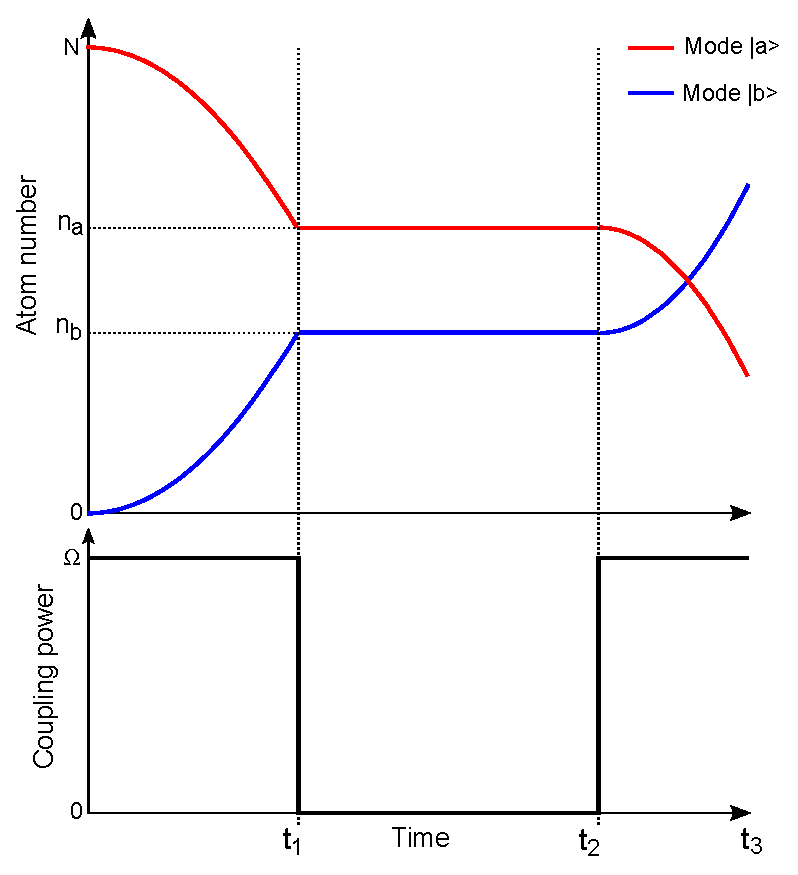
\includegraphics[width=8cm]{figures/pulse_scheme.eps}
    \caption{Schematic of the pulse sequence and atomic populations as a function of time.  Typically the coupling sequences at the beginning and end of the sequence are much shorter than the hold time, $\tau_{\mathrm{hold}} = t_2 - t_1 $, which is where the majority of the squeezing occurs. \textbf{Unless I just lied}.}
    \label{figPulseScheme}
\end{figure}

This system can be solved analytically, and expressions for quadrature, absolute and relative number squeezing can be derived. We present the solutions here; the full derivation can be found in \ref{appendixTwoModeDerivation}.
If we define
\begin{eqnarray}
s &=& \sin(\Omega (t_3 - t_2)) \label{eqsDef} \\
c &=& \cos(\Omega (t_3 - t_2)) \\
\lambda_{ij} &=& \chi_{ij} \tau_{\mathrm{hold}} / \hbar \\
A &=& \sqrt{n_a} \exp [n_a (e^{-i(\lambda_{aa}-\lambda_{ab})} - 1 )] \\
A_2 &=& n_a \exp [n_a (e^{-2i(\lambda_{aa}-\lambda_{ab})} - 1 )] \\
B &=& -i e^{i \phi}\sqrt{n_b} \exp [n_b (e^{-i(\lambda_{bb}-\lambda_{ab})} - 1 )] \\
B_2 &=& -n_b e^{2i\phi} \exp [n_b (e^{-2i(\lambda_{bb}-\lambda_{ab})} - 1 )] \\
D &=& AB^* - A^*B \label{eqDDef}
\end{eqnarray}
then the expectation values for number, number variance, and number difference variance after appling the final coupling field for a time $\tau = t_3-t_2$ are given by
\begin{eqnarray}
N_a(t_3) &=& n_a c^2 + n_b s^2 + i c s D \\
%
N_b(t_3) &=& n_a s^2 + n_b c^2 - i c s D \\
%
{\mathrm{Var}} [ N_a](t_3) &=& n_a c^2 + n_b s^2 + 2 n_a n_b c^2 s^2 \\
       && + c^2 s^2 (D^2 - e^{i(\lambda_{aa} - \lambda_{bb})} B_2 A_2^* - e^{-i(\lambda_{aa} - \lambda_{bb})} B_2^* A_2) \nonumber \\
       && + i c s D (1-2 n_a c^2 -2 n_b s^2)  \nonumber\\
       && + 2 i c^3 s n_a (e^{-i(\lambda_{aa} - \lambda_{ab})} A B^* - e^{i(\lambda_{aa} - \lambda_{ab})} A^* B ) \nonumber \\
       && + 2 i c s^3 n_b (e^{i(\lambda_{bb} - \lambda_{ab})} A B^* - e^{-i(\lambda_{bb} - \lambda_{ab})} A^* B ) \nonumber\\
%
{\mathrm{Var}} [ N_b](t_3) &=&  n_a s^2 + n_b c^2 + 2 n_a n_b c^2 s^2 \nonumber \\
       && + c^2 s^2 (D^2 - e^{i(\lambda_{aa} - \lambda_{bb})} B_2 A_2^* - e^{-i(\lambda_{aa} - \lambda_{bb})} B_2^* A_2 ) \nonumber \\
       && + i c s D (-1+2 n_a s^2 + 2 n_b c^2)  \nonumber \\
       && + 2 i c^3 s n_b (e^{-i(\lambda_{bb} - \lambda_{ab})} A^* B - e^{i(\lambda_{bb} - \lambda_{ab})} A B^* ) \nonumber \\
       && + 2 i c s^3 n_a (e^{i(\lambda_{aa} - \lambda_{ab})} A^* B - e^{-i(\lambda_{aa} - \lambda_{ab})} A B^* ) \\
%
{\mathrm{Var}} [ N_a - N_b](t_3) &=& n_a + n_b + 4 i c s D (n_a - n_b)(s^2 - c^2) \nonumber \\
       && + 4 c^2 s^2 (2 n_a n_b +D^2 - e^{i(\lambda_{aa} - \lambda_{bb})} A_2^* B_2 - e^{-i(\lambda_{aa} - \lambda_{bb})} A_2 B_2^* ) \nonumber \\
       && + 4 i c s (c^2 - s^2) (n_a e^{-i(\lambda_{aa} - \lambda_{ab})} A B^* - n_a e^{i(\lambda_{aa} - \lambda_{ab})} A^* B 
                     + n_b e^{-i(\lambda_{bb} - \lambda_{ab})} A^* B - n_b e^{i(\lambda_{bb} - \lambda_{ab})} A B^*) \label{eqNumDiffVariance}
\end{eqnarray}
In the case where all the nonlinearities are equal, such that $\chi_{aa} = \chi_{ab} = \chi_{bb}$, the number variances all reduce to those of a coherent state, e.g. ${\mathrm{Var}}[N_a]=N_a$, and no number squeezing is possible. 

While there are three independent nonlinearities $\chi_{ij}$ in the Hamiltonian (\ref{eqTwoModeHamiltonian}), the expressions for the number variances only depend on differences.  This means that number squeezing is parameterised by only two independent quantities, for example $\chi_{aa}-\chi_{ab}$ and $\chi_{aa}-\chi_{bb}$.  

{\bf{There seems to be this bogus rule of thumb in the literature that the amount of squeezing you can get is related to $\chi_{11}+\chi_{22}-2\chi_{12}$. Is it worth pointing out that this is wrong?  Joe:  Absolutely, but this might be true in some kind of weak squeezing limit, so we should check for some reference to this in the literature.}}
%Can Uaa + Ubb - 2Uab be zero and still get squeezing? Yep, Uaa=0.03, Ubb=0.01, Uab=0.2 gives squeezing for all quantities of interest

While the analytic expressions for the number variances are not particularly edifying, it is easy to evaluate and plot them for any given set of parameters. As an example, in Figure \ref{figTwoModeAnalyticExamples} we plot the solution for the normalized number variance in mode $|a\rangle$ for a particular set of nonlinearities, choosing a number of different values of $\phi$. The plots illustrate the basic features of the problem: During the final coupling period, the normalised number variance undergoes cyclic variation with a period $\tau=0.5 \Omega$, and has a series of minima. It is necessary to choose both the correct phase $\phi$ as well as the correct length of time for the coupling to be applied in order to obtain optimum squeezing.

\begin{figure}
    \centering
    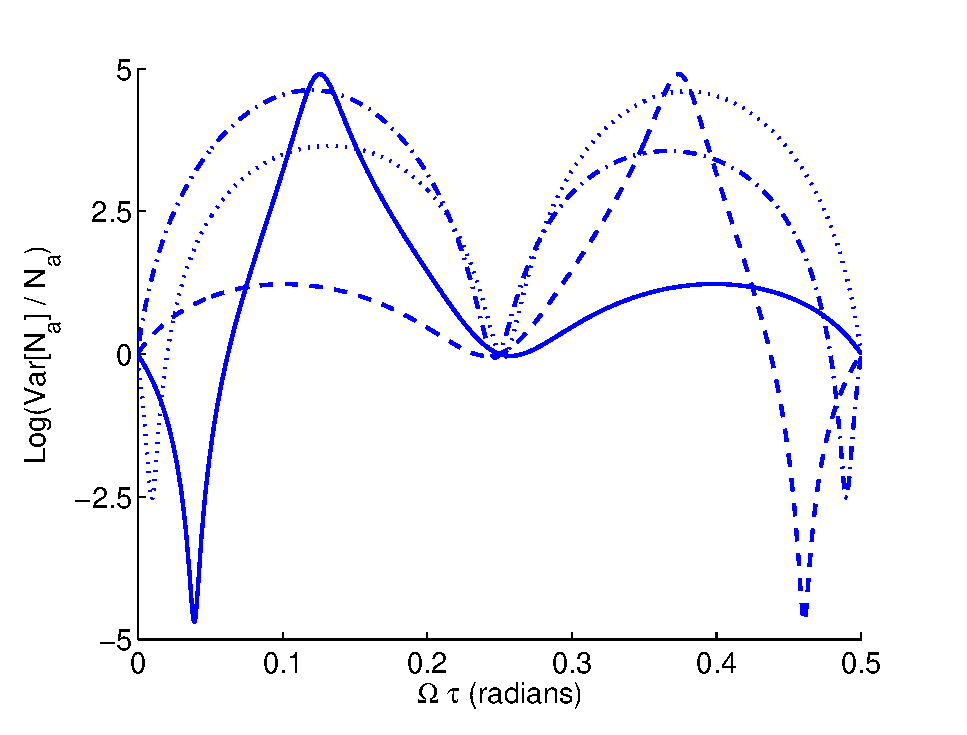
\includegraphics[width=10cm]{figures/analytic_two_mode_examples.eps}
    \caption{Normalized number variance Var$[N_a]/N_a$ in mode $\hat{a}$ as a function of final recombination time plotted on a logarithmic scale, using four different mixing angles $\phi$. Parameters: $n_a = n_b =5 \times 10^5$, $\chi_{aa}=0.04 \hbar, \chi_{ab}=0, \chi_{bb}=0.01\hbar, \tau_{\mathrm{hold}}=4\times 10^{-4}$s. Solid line, $\phi=0.10$; dash-dotted line, $\phi=1.42$; dashed line, $\phi=3.24$; dotted line, $\phi=4.71$. These particular parameters yield 21dB of number squeezing for the $\phi=0.1$ and $\phi=1.42$ cases.} 
    \label{figTwoModeAnalyticExamples}
\end{figure}


\section{Multimode analysis of squeezing}

The zero-dimensional, two-mode model described in the previous section shows that arbitrarily high squeezing can be achieved using the intrinsic nonlinearities in a BEC, but it ignores the existence of multiple spatial modes.  There are three problems caused by the existence of multiple modes, and these will limit the achievable squeezing.

The first problem is present even if the spatial modes are uncoupled.  The two-mode model shows that the parameters required to obtain best squeezing are dependent on the strength of the nonlinearity.  This nonlinearity is a function of the mode shape and the number of atoms in that mode.  The optimum hold time $\tau_{\mathrm{hold}}$ depends on this product, as does the recombination phase $\phi$.  Different modes in a multimode environment will typically have varying products of nonlinearity and therefore squeeze at different rates, with each mode having a different optimum $\tau_{\mathrm{hold}}$ and optimum recombination phase $\phi$.  This means that the best squeezing will be achieved by choosing values of $\tau_{\mathrm{hold}}$ and $\phi$ that, averaged across the range of densities, result in an overall lowest possible total number variance.  

The second problem is due to the number-dependent dynamics of the spatial modes, which is observable even in a semiclassical simulation.  Due to the nonlinear term in the Hamiltonian, the local phase evolution of the atomic field is density dependent.  Consequently the mode shape of the atomic field changes depending on the nonlinearity-density product, which means that unless $U_{aa}|\psi_a({\mathbf{r}})|^2 = U_{bb}|\psi_b({\mathbf{r}})|^2$ for all ${\mathbf{r}}$, the mode shapes will not overlap perfectly during the final coupling pulse. This degraded mode-matching will result in lower efficiency in converting the quadrature squeezing to number squeezing. We show an example of this effect in Figure~\ref{figXXX}.

\textbf{give a plot of the mode in $|a\rangle$ and $|b\rangle$ at the beginning and end of the hold time to show mismatch}

We might speculate that the effects of these first two problems would be lessened by trap geometries that lead to near-constant density profiles for the BEC.  This should enable higher squeezing.  We cannot make strong conclusions without also considering the effects of coupling between spatial modes, however.  The third potential problem is that coupling between modes is inevitable in the presence of a nonlinearity.  Coupling between modes will disturb mode-matching, and mix fields with different phase evolution, which can rapidly destroy squeezing.  

An analytic solution to the higher dimensional problem is intractable, so we must use a numerical solution.  We use stochastic methods based on phase space representations to simulate the dynamics of the multimode quantum fields.  These methods alleviate the problem of directly simulating elements of the Hilbert space, the size of which increases exponentially with the number of spatial modes \cite{stochasticRefs}.  Stochastic methods achieve this by finding a sufficiently well-behaved quasi-probability representation for the density matrix, which can then be simulated as the average behaviour of a number of low-dimensional samples.  These sample objects are the same size as the equivalent classical field.  In our case, the only tractable phase space representation is the functional Wigner representation, which is well behaved when the quantum field is approximately Gaussian, as it is for coherent and squeezed states.  Stochastic methods based on the functional Wigner representation have been used to model atom laser behaviour \cite{atomLaserWigner}, example2 \cite{example2Wigner}, and example3 \cite{example3Wigner}.

The equation of motion for the density matrix is defined by the Hamiltonian in Eq.~(\ref{eqFieldHamiltonian}).  This defines the evolution of the functional Wigner distribution of the system, which has a one-to-one correspondence with the density matrix.  The equation of motion for the functional Wigner distribution contains derivatives of third order which we assume to be negligible.  This uncontrolled approximation is called the Truncated Wigner Approximation (TWA), and while it has been used widely on ultracold gases \cite{atomlaserWigner,orOtherUCGWigner}, care must be taken that the simulation remains valid.  \textbf{Here we insert "all the checks I've done to make sure Wigner holds over the parameters we've simulated"}

Under the TWA, the equation of motion for the functional Wigner distribution is a Fokker-Planck equation, and can therefore be sampled by a set of stochastic equations, as described in \cite{GardinerQuantumNoise}.  These stochastic fields $\phi(\mathbf{x})$ are related to field operator expectation values by  
\begin{equation}
\langle :\hat{\psi}^\dagger(\mathbf{x_1})\cdots\hat{\psi}^\dagger(\mathbf{x_n})\hat{\psi}(\mathbf{y_1})\cdots\hat{\psi}(\mathbf{y_m}):_{\mbox{sym}}\rangle = \mathbb{E}\left[\phi^*(\mathbf{x_1})\cdots\phi^*(\mathbf{x_n})\phi(\mathbf{y_1})\cdots\phi(\mathbf{y_m})\right]
\label{eqExpectationRelations}
\end{equation}
%
where $:\star:_{\mbox{sym}}$ denotes symmetric ordering of the operators, and $\mathbb{E}$ denotes a stochastic average over the variables $\phi(\mathbf{x})$.  While we see below that the evolution of these fields is deterministic, the initial state still requires a random element, so multiple realisations are required.  When approximating these equations on a discrete grid, the magnitude of initial noise, the relationship between stochastic averages and the expectation values, and the equations of motion all become grid-dependent.  This is less concerning as it may at first appear, as the Hamiltonian in Eq.~(\ref{eqFieldHamiltonian}) assumes a contact potential between the atoms, and this is not correct below a length scale that can probe the details of the true potentials.  Furthermore, well before that regime is reached, the different elements of grid dependence cancel out to give grid-independent predictions for physical observables.

These stochastic equations take the form:
\begin{eqnarray}
\frac{d \phi_a}{dt} = -\frac{i}{\hbar}\left(-\frac{\hbar^2}{2 m}\nabla^2+V_a(\mathbf{x}) + U_{a a} \left|\phi_{a}\right|^2 + \frac{U_{a b}}{2} \left|\phi_b\right|^2\right)\phi_a   + \kappa \phi_b  \nonumber \\
\frac{d \phi_b}{dt} = -\frac{i}{\hbar}\left(-\frac{\hbar^2}{2 m}\nabla^2+V_b(\mathbf{x}) + U_{b b} \left|\phi_{b}\right|^2 + \frac{U_{a b}}{2} \left|\phi_a\right|^2\right)\phi_b   + \kappa^* \phi_a
  \label{eqStochasticEquations}
\end{eqnarray}
\textbf{I believe we have some rotation terms to include and explain.  Explanation can link to paragraph above}.

\textbf{Note the initial state we use, and the equations.}

We integrate equation (\ref{eqStochasticEquations}) numerically in one, two and three spatial dimensions using the numerical package XMDS \cite{Dennis2012}.  The dimensional reduction is achieved by estimating the mode shape in three dimensions, and using dimensionally reduced values for $U_{ij}$ that match the zero-dimensional reduction given by Eq.~(\ref{eqChiUequivalence}).  An equivalent process is to match the chemical potentials of the initial states.  

\section{Effects of trap geometries on squeezing in 1D}

A one-dimensional simulation is sufficient to examine the hypothesis that the squeezing will be higher for a BEC where the spatial mode has a more constant density profile.  We compare squeezing for fields starting in the ground states of a harmonic trap with negligible nonlinearity (a Gaussian), a harmonic trap with strong nonlinearity (Thomas-Fermi), and a constant potential (constant density). Using (\ref{eqChiUequivalence}) we find the following equivalences
\begin{eqnarray}
\chi &=& U \sqrt{\frac{m^3 \omega_x \omega_y \omega_z}{8 \pi^3 \hbar^3}} \,\,\,\, ({\textrm{Gaussian}}) \\
%
\chi &=& \frac{4}{7} \left( \frac{15 U \omega_x \omega_y \omega_z}{16 \pi \sqrt{2}} \right)^{2/5} \left( \frac{m}{N} \right)^{3/5} \,\,\,\, ({\textrm{Thomas-Fermi}}) \\
%
\chi &=& \frac{U}{V} \,\,\,\, {\textrm{(constant density)}}
\end{eqnarray}
\textbf{Choosing parameters where the mode shape of the multimode system doesn't change much during the evolution allows us to compare the effect of mode shape on the best squeezing that can be attained relative to the two mode system.  Joe: We need to be more specific here.} 

The results of this simulation are shown in Figure~\ref{figModalSqueezingEffects1D}, which clearly confirms the hypothesis that . Clearly the closer the mode shape is to constant density, the better.

\begin{figure}
    \centering
    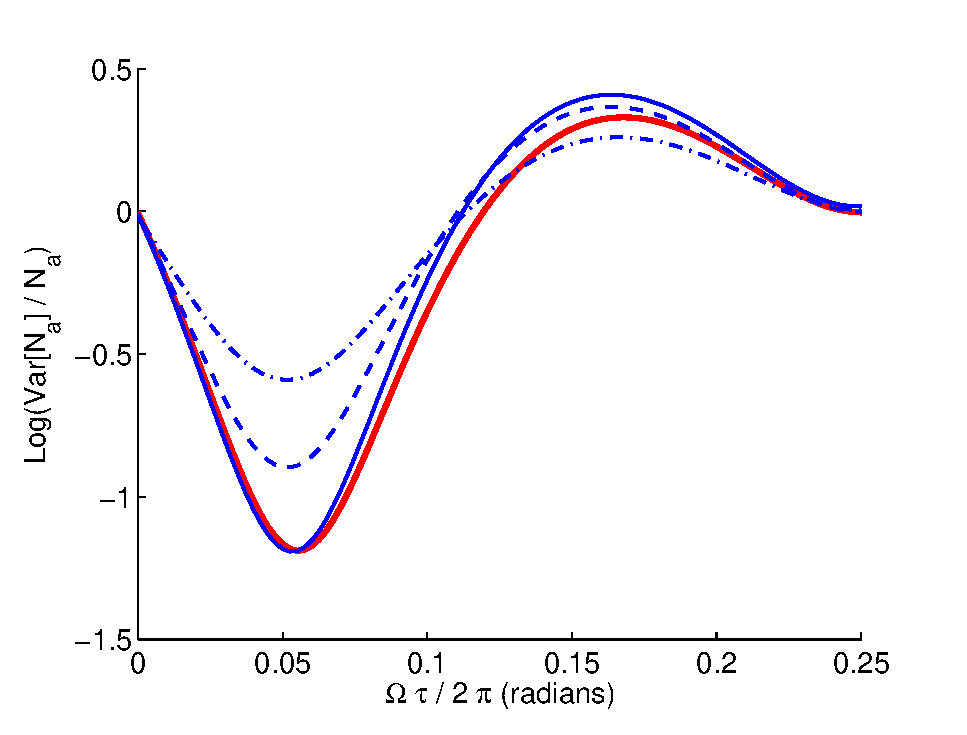
\includegraphics[width=8cm]{figures/modal_squeezing_effects_1D.eps}
    \caption{Effects of mode shape on squeezing. The plot shows the normalized number variance in mode $\hat{a}$ as a function of the time the final coupling pulse is applied. Thick red line, analytic two-mode solution; solid blue line, constant density mode; dashed line, Thomas-Fermi mode; dash-dotted line, Gaussian mode. The nonlinearities of the various 1D simulations have been adjusted for their mode shape so that they are equivalent to that of the 0D, two-mode mode nonlinearity. Parameters: $n_a = n_b =1 \times 10^5$, $\chi_{aa}=0.03 \hbar, \chi_{ab}=\chi_{bb}=0, \tau_{\mathrm{hold}}=3\times 10^{-4}$s, $\phi=4.0$. }
    \label{figModalSqueezingEffects1D}
\end{figure}

As it can be difficult to engineer specific mode shapes, another alternative is to post-select a mode. For example, rather than considering the variance in the total number of atoms in a mode, it may be possible to only count, say the atoms in the central portion of the atomic cloud. For example, suppose one had a gaussian atomic distribution, but one considers a mode that only includes the atoms within $p$ standard deviations of the centre. For low $p$, this mode shape is considerably closer to the constant density case than a standard gaussian. The equivalence between the single mode case and this mode is given by
\begin{equation}
\chi = U \frac{{\mathrm{Erf}} (\sqrt{2p})^3}{{\mathrm{Erf}}(p)^6} \sqrt{\frac{m^3 \omega_x \omega_y \omega_z}{8 \pi^3 \hbar^3}}
\end{equation}
And example comparing the best attainable squeezing for this mode compared to a single gaussian is shown in Figure~\ref{XXX}.


\section{Using a $\pi$ pulse to improve mode-matching}
\begin{itemize}
  \item Say we can use a pi pulse to swap the populations half way through, so if the states have different nonlinearities we still end up with the same mode shapes when we recombine. The fact that this works will be clear from the SM equations for a(t), b(t) when the beam splitter is on
  \item show some plots of squeezing with and without the pi pulse
\end{itemize}

\section{Squeezing in 2D and 3D}
  \begin{itemize}
  \item Two issues. 1) as we add dimensions results get worse (maybe point out how cool we are for being able to do multimode 3D simulations). 2) As our volume increases results get worse.
  \item To gain insight into this we do a bog analysis
  \item Do a comparision plot between SM analytic model and Bog to show everything agrees
  \item show that the number of mode available degrades squeezing
  \item Plot some bog results v MM sims for increasing box sizes, and increasing dimensions
  \item Can we put some numbers on how bad 3D is compared to 2D, in order to motivate tight trapping?
  \end{itemize}

\begin{figure}
  \centering
  \begin{subfigure}{.5\textwidth}
    \centering
    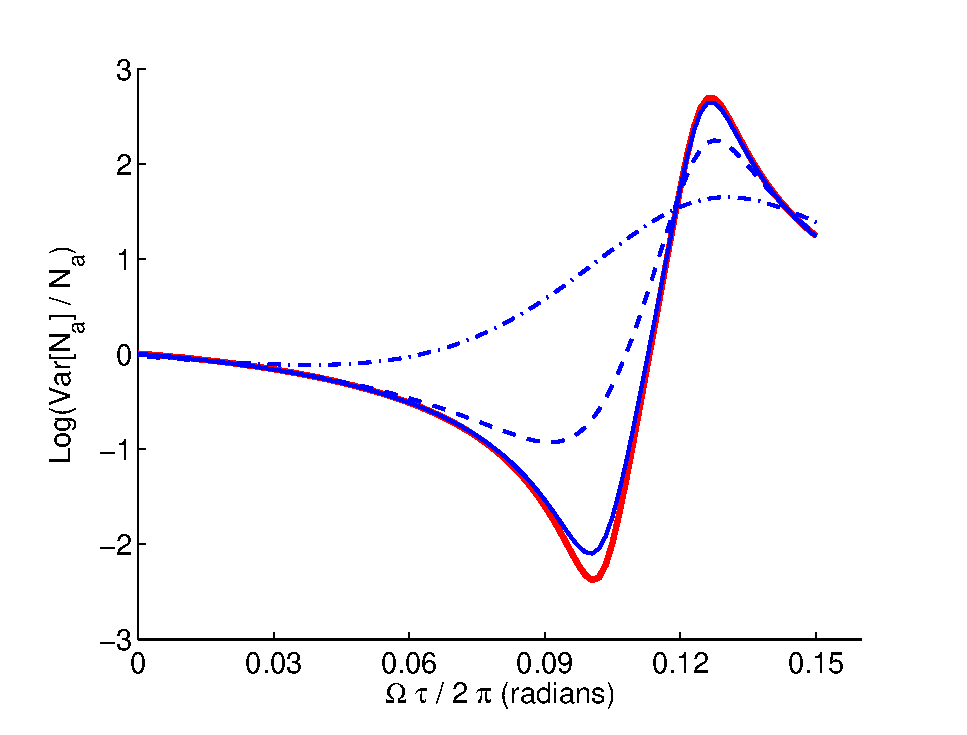
\includegraphics[width=7cm]{figures/dimensional_effects_on_squeezing_1.eps}
    \label{figDimensionalSqueezingEffects:sub1}
  \end{subfigure}%
  \begin{subfigure}{.5\textwidth}
    \centering
    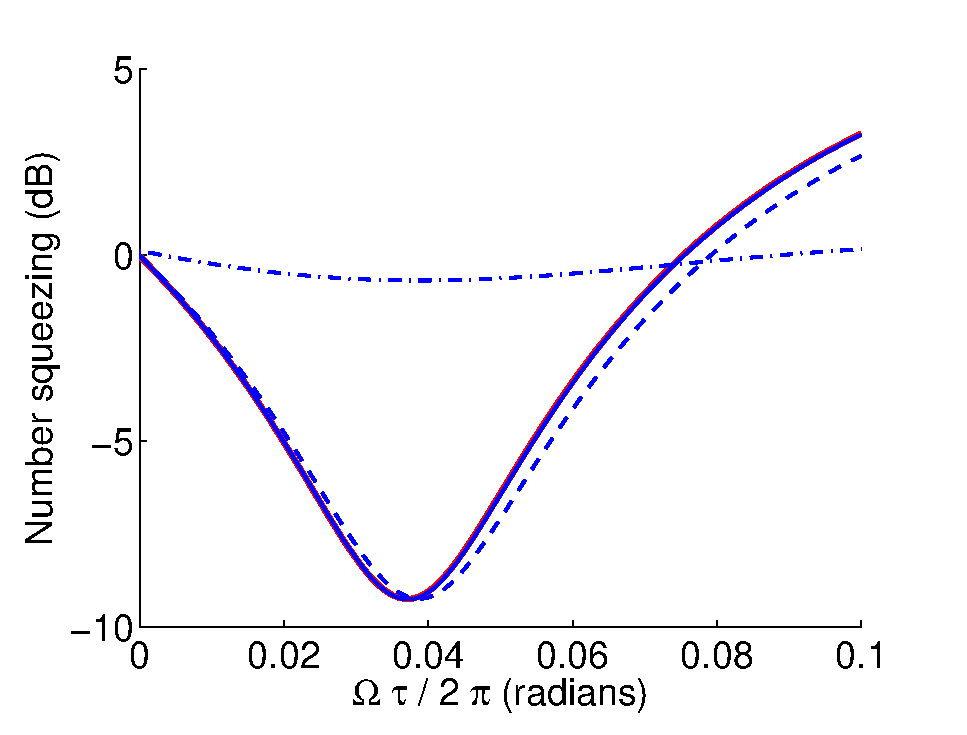
\includegraphics[width=7cm]{figures/dimensional_effects_on_squeezing_2.eps}
    \label{figDimensionalSqueezingEffects:sub2}
  \end{subfigure}
\caption{Effects of dimension on squeezing in two different nonlinear regimes. If two nonlinearities are non-zero, the deleterious effects of higher dimensions on squeezing are exacerbated. Thick red line, analytic two-mode solution; solid blue line, 1D; dashed line, 2D; dash-dotted line, 3D. (a) Parameters: $n_a = n_b =2 \times 10^5$, $\chi_{aa}=\chi_{bb}=0.03\hbar$, $\chi_{ab}=0$, $\tau_{\mathrm{hold}}=3\times 10^{-4}$s, $\phi=3.1$. (b) $n_a = n_b =2 \times 10^5$, $\chi_{aa}=0.03\hbar$, $\chi_{bb}=\chi_{ab}=0$, $\tau_{\mathrm{hold}}=3\times 10^{-4}$s, $\phi=3.1$.}
  \label{figDimensionalSqueezingEffects}
\end{figure}



\section{Mitigating multimode quantum statistical effects}
  \begin{itemize}
  \item One way to approximate constant density is to look at core of BEC, since if we only look at number in the central 1 sigma portion of gaussian it's close to flat; show results compared to single mode equivalent

  \item Another improvement is to put the BEC in a box since then we get constant density, discuss feasibility
  \item 3D still sucks even with box, so point out we can win by freezing out dimensions
  \item Show derivation for what physical situations are needed to freeze out 1, 2 and 3 dimensions. In general we need small number, which makes it hard since we want large number squeezing. Large number requirement leads to implausible geometry in 1D (i.e. a tube with a ridiculous aspect ratio), but going from 3D down to 2D is probably do-able
  \end{itemize}

In order to reduce the number of modes available, we can attempt to make our system single mode in one or more dimensions. To do this we need to ensure that that any excitation along that dimension is energetically impossible, so we always stay in the ground state. This in turn means we need the harmonic oscillator energy per particle to be greater than the nonlinear energy per particle. {\bf{*** Not happy with this explanation. Make it better ***}}.

The criteria we need to accomplish this depends on the number of dimensions we want to freeze out, so investigate the cases where we reduce a 3D system to an effective 0D, 1D, and 2D system seperately. In all cases we assume we have a box potential with length $L$ in the dimension(s) that aren't frozen out, and tight harmonic trapping potential of frequency $\omega$ in the frozen dimensions.

Reduction from 3D to 0D: Here we have tight trapping along all three dimensions, so we have a harmonic oscillator wavefunction along all dimensions. With $N$ particles in the system, the density is given by
\begin{equation}
|\psi|^2 = N \left( \frac{m \omega}{\pi \hbar} \right)^{3/2} \exp \left[ -\frac{m \omega} {\hbar} (x^2 +y^2+z^2) \right] .
\end{equation}
In this system, the nonlinear energy per particle is
\begin{eqnarray}
E_{NL} &=& \frac{U}{2N} \int |\psi({\mathbf{r}})|^4 dx \, dy \, dz \\
       &=& \frac{U N}{4 \sqrt{2}} \left( \frac{m \omega}{\pi \hbar} \right)^{3/2}
\end{eqnarray}
where $U = \pi \hbar^2 a/m$ and $a$ is the s-wave scattering length of the particles. The criterion $\hbar \omega > E_{NL}$ thus becomes
\begin{equation}
%N < \frac{1}{a} \sqrt{2 \pi \hbar}{m \omega}.
\sqrt{\frac{\hbar}{m \omega}} > \frac{aN}{\sqrt{2 \pi}}.
\end{equation}
Assuming Rubidium atoms, typical scattering lengths ($a\sim$10nm) and large particle numbers (say $N\sim 10^6$), we require a harmonic oscillator length $\sqrt{\hbar/ m \omega}>4$mm.  A BEC that's more than a centimetre across isn't particularly feasible.

Reduction from 3D to 1D: Here we have tight trapping along $x$ and $y$, with a box potential along $z$. With $N$ particles in the system, the density is given by
\begin{equation}
|\psi|^2 = \frac{N}{L} \frac{m \omega}{\pi \hbar} \exp \left[ -\frac{m \omega} {\hbar}  (x^2 +y^2) \right] .
\end{equation}
In this system, the nonlinear energy per particle is
\begin{eqnarray}
E_{NL} &=& \frac{U}{2N} \int |\psi({\mathbf{r}})|^4 dx \, dy \, dz \\
       &=& \frac{U N m \omega}{4 \pi \hbar L}
\end{eqnarray}
The criterion $\hbar \omega > E_{NL}$ thus becomes
\begin{equation}
L > a N / \pi.
\end{equation}
Assuming Rubidium atoms, typical scattering lengths ($a\sim$10nm) and large particle numbers (say $N\sim 10^6$) we need a BEC that's a few millimeters long, which isn't particularly feasible.

Reduction from 3D to 2D: Here we have tight trapping along $z$, with a box potential along $x$ and $y$. With $N$ particles in the system, the density is given by
\begin{equation}
|\psi|^2 = \frac{N}{L^2} \left( {\frac{m \omega}{\pi \hbar}} \right) ^{1/2} \exp \left[ -\frac{m \omega} {\hbar} z^2  \right]
\end{equation}
In this system, the nonlinear energy per particle is
\begin{eqnarray}
E_{NL} &=& \frac{U}{2N} \int |\psi({\mathbf{r}})|^4 dx \, dy \, dz \\
       &=& \frac{m \omega U N}{4 \pi \hbar L^2}
\end{eqnarray}
The criterion $\hbar \omega > E_{NL}$ thus becomes
\begin{equation}
\omega > \frac{8 \pi a^2 N^2 \hbar}{m L^4}.
\end{equation}
Once again taking a Rubidium atom and considering typical parameters, say $a\sim$10nm, $N\sim 10^6$, $L\sim 200\mu$m, we see that we need $\omega > 2\pi\times 190$Hz, which is feasible.

The takeaway point is that dimensional reduction to 0D and 1D is possible in the case where we have low particle numbers, which is how Oberthaler got his 6dB (or 8dB depending how you count) of squeezing. He only had 400 atoms, so could reduce his problem to 0D and freeze out any multimode dynamics. But if we're interested in large number squeezing, the best we can really do is reduction from 3D to 2D.



\section{Conclusion}
\label{sectionConclusion}
\begin{itemize}
  \item Kerr nonlinearities can give arbitrarily good squeezing in BECs with high number
  \item In a straightforward approach we can't get good squeezing with high number due to MM effects
  \item Mode matching issues can be solved with equal scattering lengths or a pi pulse or a box
  \item Another MM effect scales with dimension and physical size
  \item Can solve that problem with tight trapping and box
\end{itemize}

\ack
Acknowledgements in here; funding sources etc

\clearpage

\appendix
\section{Derivation of two mode squeezing formula}
\label{appendixTwoModeDerivation}
In this Appendix we derive the equations for the number variances which were earlier stated without proof. We use the model described in Section \ref{secTwoModeAnalytic}, where we consider a two mode system with $N$ particles, initially prepared as a coherent state with all the population in mode $|a\rangle$ at time $t=0$. A coupling pulse is then applied, so that the system evolves under the Hamiltonian
\begin{equation}
\hat{H_1} = \hbar \omega \hat{a}^{\dagger} \hat{a} +  \hbar \omega \hat{b}^{\dagger} \hat{b} 
          + \Omega (\hat{a}^{\dagger} \hat{b} + \hat{b}^{\dagger} \hat{a} )
\end{equation}
until time $t=t_1$. From time $t_1$ until time $t=t_2$ the coupling is turned off, and the system evolves under the Hamiltonian
\begin{equation}
\hat{H_2} = \frac{\chi_{aa}}{2} \hat{a}^{\dagger} \hat{a}^{\dagger} \hat{a} \hat{a}
          + \chi_{ab} \hat{a}^{\dagger} \hat{a} \hat{b}^{\dagger} \hat{b}
          + \frac{\chi_{bb}}{2} \hat{b}^{\dagger} \hat{b}^{\dagger} \hat{b} \hat{b}.
\end{equation}
Finally, from time $t_2$ until time $t=t_3$, the coupling is once again applied with a phase offset of $\phi$ relative to the first time, and the system evolves via
\begin{equation}
\hat{H_3} = \hbar \omega \hat{a}^{\dagger} \hat{a} +  \hbar \omega \hat{b}^{\dagger} \hat{b}
          + \Omega (e^{i\phi} \hat{a}^{\dagger} \hat{b} + e^{-i\phi} \hat{b}^{\dagger} \hat{a} ).
\end{equation}
It is clear that the linear self-energy terms proportional to $\omega$ result in a constant phase rotation of the fields $\hat{a}$ and $\hat{b}$. As this system is self-contained and global phase is unmeasurable, all phase measurements can only rely on the difference in phase between the two modes. This phase rotation is therefore irrelevent and will be ignored in the following analysis.

We will work in the Heisenberg picture, and derive expressions for $\hat{a}(t_3)$ and $\hat{b}(t_3)$ in terms of $\hat{a}(t_2)$ and $\hat{b}(t_2)$, which in turn can be expressed in terms of $\hat{a}(t_1)$ and $\hat{b}(t_1)$. We will show that the state of the system at time $t_1$ consists of seperate coherent states in modes $|a\rangle$ and $|b\rangle$, enabling us to calculate expectation values at time $t_3$ in terms of the known state at $t_1$.

In order to have more compact expressions we will use the notation
\begin{eqnarray}
\hat{a}(t_j) &=& \hat{a}_j \\
\hat{b}(t_j) &=& \hat{b}_j.
\end{eqnarray}

Beginning with the Hamiltonian $H_1$, during the period $(0, t_1)$ mode $\hat{a}$ will evolve as
\begin{equation}
\hat{a}_1 = e^{ i H_1 t/ \hbar} \, \hat{a}_0 \, e^{-i H_1 t/ \hbar}.
\end{equation}
Utilizing the Hadamard lemma
\begin{equation}
e^X Y e^{-X} = Y + [X,Y] + \frac{1}{2!}[X,[X,Y]] + \frac{1}{3!}[X,[X,[X,Y]]] + \ldots
\label{eqHadamard}
\end{equation}
we obtain 
\begin{eqnarray}
\hat{a}_1 &=& \hat{a}_0 - i \Omega t_1 \hat{b}_0 + \frac{(i \Omega t_1)^2}{2!} \hat{a}_0 - \frac{(i \Omega t_1)^3}{3!} \hat{b}_0 + \frac{(i \Omega t_1)^4}{4!} \hat{a}_2 - \ldots \nonumber \\
          &=& \cos (\Omega t_1) \hat{a}_0 -i \sin (\Omega t_1) \hat{b}_0.
\label{eqa1}
\end{eqnarray}
Similarly, we find
\begin{equation}
\hat{b}_1 = \cos (\Omega t_1) \hat{b}_0 - i \sin (\Omega t_1) \hat{a}_0.
\label{eqb1}
\end{equation}
From the form of (\ref{eqa1}) and (\ref{eqb1}) it is clear that as both modes $\hat{a}$ and $\hat{b}$ began in coherent states, they will remain in coherent states, with only their amplitudes changing. Specifically, at time $t_1$ the system is in a product of coherent states, which we denote $|\alpha, \beta\rangle$ with $\alpha=\sqrt{n_a}$ and $\beta=-i\sqrt{n_b}$.

Next we consider evolution under $H_2$. Taking mode $\hat{a}$ first, we note that as it commutes with the $\hat{b}^{\dagger} \hat{b}^{\dagger} \hat{b} \hat{b}$ term, and since $\hat{a}^{\dagger} \hat{a}^{\dagger} \hat{a} \hat{a}$ commutes with $\hat{a}^{\dagger} \hat{a} \hat{b}^{\dagger} \hat{b}$ we have
\begin{equation}
\hat{a}_2 = e^{i \lambda_{ab} \hat{a}_1^{\dagger} \hat{a}_1 \hat{b}_1^{\dagger} \hat{b}_1 } 
          e^{ i \frac{\lambda_{aa}} {2} \hat{a}_1^{\dagger} \hat{a}_1^{\dagger} \hat{a}_1 \hat{a}_1}\, \hat{a}_1 \,  
          e^{ -i \frac{\lambda_{aa}}{2} \hat{a}_1^{\dagger} \hat {a}_1^{\dagger} \hat{a}_1 \hat{a}_1 }
          e^{-i \lambda_{ab} \hat{a}_1^{\dagger} \hat{a}_1 \hat{b}_1^{\dagger} \hat{b}_1}
\label{eqa2evolution}
\end{equation}
where we have defined $\lambda_{ij} = \chi_{ij} (t_2-t_1)/\hbar$. Utilizing (\ref{eqHadamard}) to move $\hat{a}_1$ through the exponential, with some algebra one can show that
\begin{eqnarray}
e^{ i \frac{\lambda_{aa}} {2} \hat{a}_1^{\dagger} \hat{a}_1^{\dagger} \hat{a}_1 \hat{a}_1} \hat{a}_1 
         e^{ -i \frac{\lambda_{aa}} {2} \hat{a}_1^{\dagger} \hat{a}_1^{\dagger} \hat{a}_1 \hat{a}_1} &=& \left[ \sum_{n=0} (-i \lambda_{aa})^n (\hat{a}_1^{\dagger} \hat{a}_1)^n \right] \hat{a}_1 \nonumber \nonumber \\
   &=& \exp[-i \lambda_{aa} \hat{a}_1^{\dagger} \hat{a}_1] \hat{a}_1.
\end{eqnarray}
To handle the cross-nonlinearity term in (\ref{eqa2evolution}) we use the identity \cite{louisell}
\begin{equation}
e^{x \hat{a}^{\dagger} \hat{a}} f(\hat{a}, \hat{a}^{\dagger}) e^{-x \hat{a}^{\dagger} \hat{a}} = f(\hat{a}e^{-x}, \hat{a}^{\dagger} e^{x})
\label{eqefeidentity}
\end{equation}
to obtain
\begin{eqnarray}
\hat{a}_2 &=& e^{i \lambda_{ab} \hat{a}_1^{\dagger} \hat{a}_1 \hat{b}_1^{\dagger} \hat{b}_1 } 
          e^{-i \lambda_{aa} \hat{a}_1^{\dagger} \hat{a}_1} \, \hat{a}_1 \,
          e^{-i \lambda_{ab} \hat{a}_1^{\dagger} \hat{a}_1 \hat{b}_1^{\dagger} \hat{b}_1} \nonumber \\
%
          &=& e^{-i \lambda_{aa} \hat{a}_1^{\dagger} \hat{a}_1} 
              e^{i \lambda_{ab} \hat{a}_1^{\dagger} \hat{a}_1 \hat{b}_1^{\dagger} \hat{b}_1 } \, \hat{a}_1 \,
          e^{-i \lambda_{ab} \hat{a}_1^{\dagger} \hat{a}_1 \hat{b}_1^{\dagger} \hat{b}_1} \nonumber \\
%
          &=& e^{-i \lambda_{aa} \hat{a}_1^{\dagger} \hat{a}_1} e^{-i \lambda_{ab} \hat{b}_1^{\dagger} \hat{b}_1} \, \hat{a}_1
\label{eqa2}
\end{eqnarray}
Similarly, from permutation symmetry, we have
\begin{equation}
\hat{b}_2 = e^{-i \lambda_{bb} \hat{b}_1^{\dagger} \hat{b}_1} e^{-i \lambda_{ab} \hat{a}_1^{\dagger} \hat{a}_1} \, \hat{b}_1.     
\label{eqb2}
\end{equation}
Finally, to obtain $\hat{a}_3$ and $\hat{b}_3$ we utilize (\ref{eqa1}) and (\ref{eqb1}) with the phase factor attached to the $\hat{b}$ operator to obtain
\begin{eqnarray}
\hat{a}_3 &=& \cos (\Omega (t_3-t_2)) \hat{a}_2 -i e^{i\phi} \sin (\Omega (t_3-t_2)) \hat{b}_2 \label{eqa3} \\
\hat{b}_3 &=& \cos (\Omega (t_3-t_2)) \hat{b}_2 - i e^{-i\phi} \sin (\Omega (t_3-t_2)) \hat{a}_2 \label{eqb3}
\end{eqnarray} 
We are now in a position to evaluate the number variance of the system throughout the period of the final coupling. The number variances of the fields are defined as
\begin{eqnarray}
{\mathrm{Var}}[N_a] &=& \langle \hat{a}^{\dagger}_3 \hat{a}_3 \hat{a}^{\dagger}_3 \hat{a}_3 \rangle - \langle \hat{a}^{\dagger}_3 \hat{a}_3 \rangle ^2 \label{eqNavariance} \\
%
{\mathrm{Var}}[N_b] &=& \langle \hat{b}^{\dagger}_3 \hat{b}_3 \hat{b}^{\dagger}_3 \hat{b}_3 \rangle - \langle \hat{b}^{\dagger}_3 \hat{b}_3 \rangle ^2.
\label{eqNbvariance}
\end{eqnarray}
Making use of (\ref{eqa3}) and using the shorthand notation 
\begin{eqnarray}
s &=& \sin[\Omega (t_3 - t_2)] \\
c &=& \cos[\Omega (t_3 - t_2)]
\end{eqnarray}
we have
\begin{eqnarray}
\hat{a}^{\dagger}_3 \hat{a}_3 &=& \hat{a}^{\dagger}_2 \hat{a}_2 c^2 +  \hat{b}^{\dagger}_2 \hat{b}_2 s^2 + i c s (e^{-i \phi} \hat{b}^{\dagger}_2 \hat{a}_2 - e^{i \phi} \hat{a}^{\dagger}_2 \hat{b}_2) \\
%
%
\hat{a}^{\dagger}_3 \hat{a}_3 \hat{a}^{\dagger}_3 \hat{a}_3 &=& \hat{a}^{\dagger}_2 \hat{a}_2 \hat{a}^{\dagger}_2 \hat{a}_2 c^4 + \hat{b}^{\dagger}_2 \hat{b}_2 \hat{b}^{\dagger}_2 \hat{b}_2 s^4 \nonumber \\
%
&& + c^2 s^2 [ \hat{a}^{\dagger}_2 \hat{a}_2 + \hat{b}^{\dagger}_2 \hat{b}_2 + 4 \hat{a}^{\dagger}_2 \hat{a}_2 \hat{b}^{\dagger}_2 \hat{b}_2 -e^{-2 i \phi} \hat{a}^{\dagger}_2 \hat{a}^{\dagger}_2 \hat{b}_2 \hat{b}_2 -e^{-2 i \phi} \hat{b}^{\dagger}_2 \hat{b}^{\dagger}_2 \hat{a}_2 \hat{a}_2 ] \nonumber \\
%
&& + i c^3 s [2 e^{-i \phi} \hat{b}^{\dagger}_2 \hat{a}^{\dagger}_2 \hat{a}_2 \hat{a}_2 - 2 e^{i \phi} \hat{a}^{\dagger}_2 \hat{a}^{\dagger}_2 \hat{a}_2 \hat{b}_2 + e^{-i \phi} \hat{b}^{\dagger}_2 \hat{a}_2 - e^{i \phi} \hat{a}^{\dagger}_2 \hat{b}_2 ] \nonumber \\
%
&& + i c s^3 [2 e^{-i \phi} \hat{b}^{\dagger}_2 \hat{b}^{\dagger}_2 \hat{a}_2 \hat{b}_2 - 2 e^{i \phi} \hat{a}^{\dagger}_2 \hat{b}^{\dagger}_2 \hat{b}_2 \hat{b}_2 + e^{-i \phi} \hat{b}^{\dagger}_2 \hat{a}_2 - e^{i \phi} \hat{a}^{\dagger}_2 \hat{b}_2 ]
\end{eqnarray}
\begin{eqnarray}
\hat{b}^{\dagger}_3 \hat{b}_3 &=& \hat{b}^{\dagger}_2 \hat{b}_2 c^2 +  \hat{a}^{\dagger}_2 \hat{a}_2 s^2 + i c s ( e^{i \phi} \hat{a}^{\dagger}_2 \hat{b}_2 - e^{-i \phi} \hat{b}^{\dagger}_2 \hat{a}_2) \\
%
%
\hat{b}^{\dagger}_3 \hat{b}_3 \hat{b}^{\dagger}_3 \hat{b}_3 &=& \hat{b}^{\dagger}_2 \hat{b}_2 \hat{b}^{\dagger}_2 \hat{b}_2 c^4 + \hat{a}^{\dagger}_2 \hat{a}_2 \hat{a}^{\dagger}_2 \hat{a}_2 s^4 \nonumber \\
%
&& + c^2 s^2 [ \hat{b}^{\dagger}_2 \hat{b}_2 + \hat{a}^{\dagger}_2 \hat{a}_2 + 4 \hat{b}^{\dagger}_2 \hat{b}_2 \hat{a}^{\dagger}_2 \hat{a}_2 - e^{2 i \phi} \hat{b}^{\dagger}_2 \hat{b}^{\dagger}_2 \hat{a}_2 \hat{a}_2 -e^{2 i \phi} \hat{a}^{\dagger}_2 \hat{a}^{\dagger}_2 \hat{b}_2 \hat{b}_2 ] \nonumber \\
%
&& + i c^3 s [2 e^{i \phi} \hat{a}^{\dagger}_2 \hat{b}^{\dagger}_2 \hat{b}_2 \hat{b}_2 - 2 e^{-i \phi} \hat{b}^{\dagger}_2 \hat{b}^{\dagger}_2 \hat{b}_2 \hat{a}_2 + e^{i \phi} \hat{a}^{\dagger}_2 \hat{b}_2 - e^{-i \phi} \hat{b}^{\dagger}_2 \hat{a}_2 ] \nonumber \\
%
&& + i c s^3 [2 e^{i \phi} \hat{a}^{\dagger}_2 \hat{a}^{\dagger}_2 \hat{b}_2 \hat{a}_2 - 2 e^{-i \phi} \hat{b}^{\dagger}_2 \hat{a}^{\dagger}_2 \hat{a}_2 \hat{a}_2 + e^{i \phi} \hat{a}^{\dagger}_2 \hat{b}_2 - e^{-i \phi} \hat{b}^{\dagger}_2 \hat{a}_2 ] 
\end{eqnarray}
Clearly, to calculate (\ref{eqNavariance}) and (\ref{eqNbvariance}) we will need the expectation values of terms quartic and quadratic in $\hat{a}_2$ and ${\hat{b}_2}$. Specifically, we require $\langle \hat{a}^{\dagger}_2 \hat{a}_2 \rangle$, $\langle \hat{b}^{\dagger}_2 \hat{b}_2 \rangle$,  $\langle \hat{a}^{\dagger}_2 \hat{b}_2 \rangle$, $\langle \hat{a}^{\dagger}_2 \hat{a}_2 \hat{a}^{\dagger}_2 \hat{a}_2 \rangle$, $\langle \hat{b}^{\dagger}_2 \hat{b}_2 \hat{b}^{\dagger}_2 \hat{b}_2 \rangle$ , $\langle \hat{a}^{\dagger}_2 \hat{a}_2 \hat{b}^{\dagger}_2 \hat{b}_2 \rangle$, $\langle \hat{a}^{\dagger}_2 \hat{a}^{\dagger}_2 \hat{b}_2 \hat{b}_2 \rangle$, $\langle \hat{a}^{\dagger}_2 \hat{b}^{\dagger}_2 \hat{a}_2 \hat{a}_2 \rangle$, and $\langle \hat{a}^{\dagger}_2 \hat{b}^{\dagger}_2 \hat{b}_2 \hat{b}_2 \rangle$, as well as their Hermitian conjugates.

As $\hat{a}^{\dagger}_1 \hat{a}_1$ and $\hat{b}^{\dagger}_1 \hat{b}_1$ commute with the Hamiltonian $H_2$, they are constants of motion so we have
\begin{equation}
\langle \hat{a}^{\dagger}_2 \hat{a}_2 \rangle = \langle \hat{a}^{\dagger}_1 \hat{a}_1 \rangle = \langle \alpha, \beta | \hat{a}^{\dagger}_1 \hat{a}_1 |\alpha, \beta \rangle = |\alpha|^2 = n_a
\end{equation}
%
\begin{equation}
\langle \hat{b}^{\dagger}_2 \hat{b}_2 \rangle = \langle \hat{b}^{\dagger}_1 \hat{b}_1 \rangle = \langle \alpha, \beta | \hat{b}^{\dagger}_1 \hat{b}_1 |\alpha, \beta \rangle = |\beta|^2 = n_b
\end{equation}
%
\begin{equation}
\langle \hat{a}^{\dagger}_2 \hat{a}_2 \hat{b}^{\dagger}_2 \hat{b}_2 \rangle = \langle \hat{a}^{\dagger}_1 \hat{a}_1 \hat{b}^{\dagger}_1 \hat{b}_1 \rangle = \langle \alpha, \beta | \hat{a}^{\dagger}_1 \hat{a}_1 \hat{b}^{\dagger}_1 \hat{b}_1 |\alpha, \beta \rangle = |\alpha|^2 |\beta|^2 = n_a n_b
\end{equation}
Furthermore, $\hat{a}^{\dagger}_2 \hat{a}_2 \hat{a}^{\dagger}_2 \hat{a}_2$ and $\hat{b}^{\dagger}_2 \hat{b}_2 \hat{b}^{\dagger}_2 \hat{b}_2$ also commute with $H_2$, giving
\begin{equation}
\langle \hat{a}^{\dagger}_2 \hat{a}_2 \hat{a}^{\dagger}_2 \hat{a}_2 \rangle = \langle \hat{a}^{\dagger}_1 \hat{a}_1 \hat{a}^{\dagger}_1 \hat{a}_1 \rangle = \langle \alpha, \beta | \hat{a}^{\dagger}_1 \hat{a}^{\dagger}_1 \hat{a}_1 \hat{a}_1 + \hat{a}^{\dagger}_1 \hat{a}_1 |\alpha, \beta \rangle = n_a^2 + n_a
\end{equation}
%
\begin{equation}
\langle \hat{b}^{\dagger}_2 \hat{b}_2 \hat{b}^{\dagger}_2 \hat{b}_2 \rangle = \langle \hat{b}^{\dagger}_1 \hat{b}_1 \hat{b}^{\dagger}_1 \hat{b}_1 \rangle = \langle \alpha, \beta | \hat{b}^{\dagger}_1 \hat{b}^{\dagger}_1 \hat{b}_1 \hat{b}_1 + \hat{b}^{\dagger}_1 \hat{b}_1 |\alpha, \beta \rangle = n_b^2 + n_b
\end{equation}
The remaining terms are not constants of motion, so we proceed by making use of (\ref{eqa2}) and (\ref{eqb2}). For $\langle \hat{a}^{\dagger}_2 \hat{b}_2 \rangle$ we have
\begin{equation}
\hat{a}^{\dagger}_2 \hat{b}_2 = \hat{a}^{\dagger}_1 e^{-i (\lambda_{bb} - \lambda_{ab}) \hat{b}^{\dagger}_1 \hat{b}_1} e^{i (\lambda_{aa} - \lambda_{ab}) \hat{a}^{\dagger}_1 \hat{a}_1} \hat{b}_1. 
\end{equation}
To calculate the expectation value of this expression, the creation and annihilation operators must be normally ordered. Making use of the identity \cite{louisell}
\begin{equation}
e^{x \hat{a}^{\dagger} \hat{a}} = \sum_{n=0}^{\infty} \frac{(e^x - 1)^n} {n!} (\hat{a}^{\dagger})^n (\hat{a})^n
\end{equation}
allows us to compute expectation values of coherent states of the form
\begin{eqnarray}
\langle \alpha | e^{x \hat{a}^{\dagger} \hat{a}} |\alpha \rangle &=& \sum_{n=0}^{\infty} \frac{(e^x - 1)^n} {n!} |\alpha|^{2n} \nonumber \\
%
&=& \exp[|\alpha|^2(e^x -1)]. \label{eqExpectationValueOfExponential}
\end{eqnarray}
This gives
\begin{eqnarray}
\langle \hat{a}^{\dagger}_2 \hat{b}_2 \rangle &=& \langle \alpha, \beta | \hat{a}^{\dagger}_1 e^{-i (\lambda_{bb} - \lambda_{ab}) \hat{b}^{\dagger}_1 \hat{b}_1} e^{i (\lambda_{aa} - \lambda_{ab}) \hat{a}^{\dagger}_1 \hat{a}_1} \hat{b}_1 | \alpha, \beta \rangle \nonumber \\
%
&=& \alpha^* \beta \exp[|\alpha|^2(e^{i (\lambda_{aa} - \lambda_{ab})} -1)] \exp[|\beta|^2 (e^{-i (\lambda_{bb} - \lambda_{ab})} -1)].
\end{eqnarray}

Next we tackle $\langle \hat{a}^{\dagger}_2 \hat{a}^{\dagger}_2 \hat{b}_2 \hat{b}_2 \rangle$. Using (\ref{eqa2}) and (\ref{eqb2}) and the fact that $\hat{a}$ and $\hat{b}$ commute, we have
\begin{eqnarray}
\hat{a}^{\dagger}_2 \hat{a}^{\dagger}_2 \hat{b}_2 \hat{b}_2 &=& \hat{a}^{\dagger}_1 
  e^{i (\lambda_{aa}-\lambda_{ab}) \hat{a}^{\dagger}_1 \hat{a}_1}
  \hat{b}_1 \hat{a}^{\dagger_1}
  e^{i (\lambda_{ab}-\lambda_{bb}) \hat{b}^{\dagger}_1 \hat{b}_1}
  e^{i (\lambda_{aa}-\lambda_{ab}) \hat{a}^{\dagger}_1 \hat{a}_1}
  \hat{b}_1 \\
%
&=& \hat{a}^{\dagger}_1 \hat{a}^{\dagger}_1 
    e^{2i (\lambda_{aa}-\lambda_{ab}) \hat{a}^{\dagger}_1 \hat{a}_1}
    e^{2i (\lambda_{ab}-\lambda_{bb}) \hat{b}^{\dagger}_1 \hat{b}_1}
    \hat{b}_1 \hat{b}_1 e^{i(\lambda_{aa}-\lambda_{bb})}
\end{eqnarray}
where we have made multiple uses of the identity 
\begin{equation}
\hat{a} e^{i x \hat{a}^{\dagger} \hat{a}} = e^{i x \hat{a}^{\dagger} \hat{a}} \hat{a} e^{ix}
\end{equation}
which follows from (\ref{eqefeidentity}). Finally, applying (\ref{eqExpectationValueOfExponential}) we obtain
\begin{equation}
\langle \hat{a}^{\dagger}_2 \hat{a}^{\dagger}_2 \hat{b}_2 \hat{b}_2 \rangle = \alpha^{*2} \beta^2 e^{i(\lambda_{aa}-\lambda_{bb})} \exp[|\alpha|^2(e^{2i (\lambda_{aa} - \lambda_{bb})} -1)] \exp[|\beta|^2(e^{-2i (\lambda_{bb} - \lambda_{bb})} -1)].
\end{equation}
Using the same techniques one can show that
\begin{eqnarray}
\langle \hat{a}^{\dagger}_2 \hat{b}^{\dagger}_2 \hat{a}_2 \hat{a}_2 \rangle &=& |\alpha|^2 \alpha \beta^* e^{-i(\lambda_{aa}-\lambda_{ab})} \exp[|\alpha|^2(e^{-i (\lambda_{aa} - \lambda_{ab})} -1)] \exp[|\beta|^2(e^{i (\lambda_{bb} - \lambda_{ab})} -1)] \\
%
\langle \hat{a}^{\dagger}_2 \hat{b}^{\dagger}_2 \hat{b}_2 \hat{b}_2 \rangle &=& |\beta|^2 \alpha^{*} \beta e^{-i(\lambda_{bb}-\lambda_{ab})} \exp[|\alpha|^2(e^{i (\lambda_{aa} - \lambda_{ab})} -1)] \exp[|\beta|^2(e^{-i (\lambda_{bb} - \lambda_{ab})} -1)].
\end{eqnarray}
Employing the definitions (\ref{eqsDef})--(\ref{eqDDef}) we obtain
\begin{eqnarray}
\langle \hat{a}^{\dagger}(t_3) \hat{a}(t_3) \rangle &=& n_a c^2 + n_b s^2 + i c s (A B^* - A^* B) \\
%
\langle \hat{b}^{\dagger}(t_3) \hat{b}(t_3) \rangle &=& n_a s^2 + n_b c^2 - i c s (A B^* - A^* B) \\
%
\langle \hat{a}^{\dagger}(t_3) \hat{a}(t_3) \hat{a}^{\dagger}(t_3)  \hat{a}(t_3) \rangle &=& (n_a^2 + n_a) c^4 + (n_b^2 + n_b) s^4 \nonumber \\
&& + c^2 s^2 [n_a +n_b +4 n_a n_b - e^{i(\lambda_{aa}-\lambda_{bb})} B_2 A_2^* - e^{-i(\lambda_{aa}-\lambda_{bb})} B_2^* A_2] \nonumber \\
&& + i c^3 s [2 n_a e^{-i(\lambda_{aa}-\lambda_{ab})}] A B^* - 2 n_a e^{i(\lambda_{aa}-\lambda_{ab})} A^* B + A B^* - A^* B] \nonumber \\
&& + i c s^3 [2 n_b e^{i(\lambda_{bb}-\lambda_{ab})}] A B^* - 2 n_b e^{-i(\lambda_{bb}-\lambda_{ab})} A^* B + A B^* - A^* B] \\
%
\langle \hat{b}^{\dagger}(t_3)  \hat{b}(t_3) \hat{b}^{\dagger}(t_3)  \hat{b}(t_3) \rangle &=& (n_b^2 + n_b) c^4 + (n_a^2 + n_a) s^4 \nonumber \\
&& + c^2 s^2 [n_a +n_b +4 n_a n_b - e^{-i(\lambda_{aa}-\lambda_{bb})} B_2^* A_2 - e^{i(\lambda_{aa}-\lambda_{bb})} B_2 A_2^*] \nonumber \\
&& + i c^3 s [2 n_b e^{-i(\lambda_{bb}-\lambda_{ab})}] A^* B - 2 n_b e^{i(\lambda_{bb}-\lambda_{ab})} A B^* - A^* B + A B^*] \nonumber \\
&& + i c s^3 [2 n_a e^{i(\lambda_{aa}-\lambda_{ab})}] A^* B - 2 n_a e^{-i(\lambda_{aa}-\lambda_{ab})} A B^* - A^* B + A B^*]. 
\end{eqnarray}
When substituted into (\ref{eqNavariance}) and (\ref{eqNbvariance}) these expecation values give the absolute number variances stated in Section \ref{secTwoModeAnalytic}. To calculate the number difference variance, we note
\begin{equation}
{\mathrm{Var}}[N_a-N_b] = {\mathrm{Var}}[N_a] + {\mathrm{Var}}[N_b] - 2\langle \hat{a}^{\dagger}_3 \hat{a}_3 \hat{b}^{\dagger}_3 \hat{b}_3\rangle + 2\langle \hat{a}^{\dagger}_3  \hat{a}_3 \rangle \langle \hat{b}^{\dagger}_3 \hat{b}_3\rangle \label{eqNumDiffVarianceAppendix}.
\end{equation}
We write (\ref{eqNumDiffVarianceAppendix}) in terms of $\hat{a}_2$ and $\hat{b}_2$ by using using (\ref{eqa3}) and (\ref{eqb3}), and then use the expectation values calculated earlier in this Appendix. After some algebra we obtain the expression (\ref{eqNumDiffVariance}) given in Section \ref{secTwoModeAnalytic}.



\section*{References}
\begin{thebibliography}{10}
\bibitem{gross2010} Gross C, Zibold T, Est{\`{e}}ve J and Oberthaler M K 2010 Nonlinear atom interferometer surpasses classical
precision limit {\it Nature} {\bf 464} 1165--1169
\bibitem{dennis2013} Dennis G R, Hope J J and Johnsson M T 2013 XMDS2: Fast, scalable simulation of coupled stochastic partial
differential equations {\it Comput. Phys. Commun.} {\bf 184} 201--208
\bibitem{louisell} Louisell Quantum Statistical Properties of Radiation
\end{thebibliography}

\end{document}

